%\documentclass[
  bibliography=totoc,     % Literatur im Inhaltsverzeichnis
  captions=tableheading,  % Tabellenüberschriften
  titlepage=firstiscover, % Titelseite ist Deckblatt
]{scrartcl}

% Paket float verbessern
\usepackage{scrhack}

% Warnung, falls nochmal kompiliert werden muss
\usepackage[aux]{rerunfilecheck}

% unverzichtbare Mathe-Befehle
\usepackage{amsmath}
% viele Mathe-Symbole
\usepackage{amssymb}
% Erweiterungen für amsmath
\usepackage{mathtools}

% Fonteinstellungen
\usepackage{fontspec}
% Latin Modern Fonts werden automatisch geladen
% Alternativ zum Beispiel:
%\setromanfont{Libertinus Serif}
%\setsansfont{Libertinus Sans}
%\setmonofont{Libertinus Mono}

% Wenn man andere Schriftarten gesetzt hat,
% sollte man das Seiten-Layout neu berechnen lassen
\recalctypearea{}

% deutsche Spracheinstellungen
\usepackage[ngerman]{babel}


\usepackage[
  math-style=ISO,    % ┐
  bold-style=ISO,    % │
  sans-style=italic, % │ ISO-Standard folgen
  nabla=upright,     % │
  partial=upright,   % │
  mathrm=sym,        % ┘
  warnings-off={           % ┐
    mathtools-colon,       % │ unnötige Warnungen ausschalten
    mathtools-overbracket, % │
  },                       % ┘
]{unicode-math}

% traditionelle Fonts für Mathematik
\setmathfont{Latin Modern Math}
% Alternativ zum Beispiel:
%\setmathfont{Libertinus Math}

\setmathfont{XITS Math}[range={scr, bfscr}]
\setmathfont{XITS Math}[range={cal, bfcal}, StylisticSet=1]

% Zahlen und Einheiten
\usepackage[
  locale=DE,                   % deutsche Einstellungen
  separate-uncertainty=true,   % immer Unsicherheit mit \pm
  per-mode=symbol-or-fraction, % / in inline math, fraction in display math
]{siunitx}

% chemische Formeln
\usepackage[
  version=4,
  math-greek=default, % ┐ mit unicode-math zusammenarbeiten
  text-greek=default, % ┘
]{mhchem}

% richtige Anführungszeichen
\usepackage[autostyle]{csquotes}

% schöne Brüche im Text
\usepackage{xfrac}

% Standardplatzierung für Floats einstellen
\usepackage{float}
\floatplacement{figure}{htbp}
\floatplacement{table}{htbp}

% Floats innerhalb einer Section halten
\usepackage[
  section, % Floats innerhalb der Section halten
  below,   % unterhalb der Section aber auf der selben Seite ist ok
]{placeins}

% Seite drehen für breite Tabellen: landscape Umgebung
\usepackage{pdflscape}

% Captions schöner machen.
\usepackage[
  labelfont=bf,        % Tabelle x: Abbildung y: ist jetzt fett
  font=small,          % Schrift etwas kleiner als Dokument
  width=0.9\textwidth, % maximale Breite einer Caption schmaler
]{caption}
% subfigure, subtable, subref
\usepackage{subcaption}

% Grafiken können eingebunden werden
\usepackage{graphicx}

% schöne Tabellen
\usepackage{tabularray}
\UseTblrLibrary{booktabs, siunitx}

% Verbesserungen am Schriftbild
\usepackage{microtype}

% Literaturverzeichnis
\usepackage[
  backend=biber,
]{biblatex}
% Quellendatenbank
\addbibresource{lit.bib}
\addbibresource{programme.bib}

% Hyperlinks im Dokument
\usepackage[
  german,
  unicode,        % Unicode in PDF-Attributen erlauben
  pdfusetitle,    % Titel, Autoren und Datum als PDF-Attribute
  pdfcreator={},  % ┐ PDF-Attribute säubern
  pdfproducer={}, % ┘
]{hyperref}
% erweiterte Bookmarks im PDF
\usepackage{bookmark}

% Trennung von Wörtern mit Strichen
\usepackage[shortcuts]{extdash}

\author{%
  Vincent Wirsdörfer\\%
  \href{mailto:vincent.wirsdoerfer@udo.edu}{authorA@udo.edu}%
  \and%
  Joris Daus\\%
  \href{mailto:joris.daus@udo.edu}{authorB@udo.edu}%
}
\publishers{TU Dortmund – Fakultät Physik}


%\begin{document}
\section{Diskussion}
\label{sec:Diskussion}

In diesem Experiment stellt die Überprüfbarkeit der Ergebnisse Herausforderungen dar. 
Das Ziel dieses Experimentes ist nicht wie im klassischen Sinne Konstanten oder Größen 
herauszufinden, sondern den Umgang und Anwendungsmöglichkeiten der Ultraschalltechnik 
zu betrachten. Es wird im Folgenden den Umständen geschuldet also mehr auf die 
Techniken als auf konkrete Werte eingegangen. 

\subsection{Abstandsmessungen mit einem Acrylblock}
Die Durchführung der Durchmessermessung hat konkret keine bemerkenswerten Schwierigkeiten 
bereitet. Die Lokalisierung der Löcher in dem Computerprogramm ist sehr eindeutig. Zur 
Verifizierung, ob der ausgewählte Peak von dem Loch stammt, wird die Ultraschallsonde 
leicht nach links und rechts verschoben. Verringert sich dann die  ausgewählte Amplitude, 
kann mit großer Sicherheit gesagt werden, dass der Peak im A-Scan von dem zu beobachtenden 
Loch stammt. Jedoch mussten bei der Auswertung annahmen getroffen werden, welche zu einer 
Ungenauigkeit in den Ergebnissen führen können. So muss die Schallgeschwindigkeit in der 
Anpassungsschicht auf die von Acryl abgeschätzt werden. Des Weiteren wäre es genauer, wenn 
die Dicke der Anpassungsschicht von vornherein bekannt wäre, sodass sich keine Fehler aus 
jener Berechnung fortpflanzen können. Außerdem wir pro Loch nur eine Messung durchgeführt. 
Dies führt dazu, dass statistische Fehler nicht ausgeglichen werden können. In der Auswertung 
wird eine Schallgeschwindigkeit in Acryl von \qty{273,78}{\meter \per \second} konstituiert. 
Verglichen mit dem Literaturwert von \qty{2730}{\meter\per\second} ist dies eine Abweichung 
von lediglich \qty{1,1}{\percent}. Dies deutet darauf hin, dass obwohl nur eine Messung pro 
Loch aufgenommen wird, dennoch sehr genaue Werte bestimmt werden. Die über die 
Schallgeschwindigkeit bestimmten Durchmesser der Löcher $D_\text{Schall}$ werden nun mit den 
über den Messchieber bestimmten Durchmesser $D_\text{Mess}$ verglichen.

\begin{table}
    \centering 
    \caption{Vergleich errechneter Durchmesser der Lochbohrungen im Acrylblock.}
    \sisetup{table-format = 2.2, separate-uncertainty=true}
    \label{tab:Durchmesser}
    \begin{tblr}{
        colspec = {S[separate-uncertainty=false, table-format=2.0] S S S S[seperate-uncertainty=true, table-format=3.2(1), table-format=2.2(2)]},
        row{1, 2, 3, 4, 5, 6, 7, 8, 9, 10, 11, 12} = {guard, mode=math},
        }
        \toprule 
        \text{Loch Nr.} & D_\text{Schall} \mathbin{/} \unit{\milli\meter} & D_\text{Mess} \mathbin{/} \unit{\milli\meter} 
        & \Delta D \mathbin{/} \unit{\milli\meter} & \Delta D \mathbin{/} \unit{\percent} \\
        \midrule 
        1   &   1.20\pm0.27 &   0.80\pm0.04 &   0.40\pm0.03 &    50.26\pm6.56   \\
        2   &   1.45\pm0.27 &   0.70\pm0.04 &   0.75\pm0.03 &   106.82\pm10.79  \\
        3   &   6.20\pm0.27 &   5.30\pm0.04 &   0.90\pm0.03 &    16.94\pm0.75   \\
        4   &   5.11\pm0.27 &   4.30\pm0.04 &   0.81\pm0.03 &    18.74\pm0.94   \\
        5   &   4.05\pm0.27 &   3.30\pm0.04 &   0.75\pm0.03 &    22.86\pm1.27   \\
        6   &   3.14\pm0.27 &   2.45\pm0.04 &   0.69\pm0.03 &    28.18\pm1.79   \\
        7   &   3.15\pm0.27 &   2.45\pm0.04 &   0.70\pm0.03 &    28.73\pm1.76   \\
        8   &   3.21\pm0.27 &   2.45\pm0.04 &   0.71\pm0.03 &    28.34\pm1.76   \\
        9   &   3.26\pm0.27 &   2.45\pm0.04 &   0.76\pm0.03 &    30.53\pm1.79   \\
        10  &   1.16\pm0.27 &   2.60\pm0.04 &   3.76\pm0.03 &   144.59\pm1.62   \\
        11  &   6.48\pm0.27 &   9.12\pm0.04 &   2.72\pm0.03 &    29.52\pm0.27   \\
        \bottomrule 
    \end{tblr}
\end{table}

\noindent Wie in der Tabelle zu erkennen, weichen die meisten Durchmmesser maximal um \qty{30}{\percent} 
zwischen den Berechnungsmethoden ab. Die Löcher Nr. 1, 2, und 10 bilden ein Ausnahme. Dies kann gegebenenfalls 
wie schon erwähnt daran liegen, dass nur eine Messung pro Loch durchgeführt wird und somit statistische 
Fehler erscheinen. Die Abweichung von meistens ungefähr \qty{0.7}{\milli \meter} kann darauf zurückgeführt 
werden, dass die Anpassungsschicht nicht genau genug berechnet worden ist. Dies wird dadurch unterstützt, 
dass der Wert der absoluten Abweichung sehr konstant ist.


\subsection{Augenmodell}
Die Vermessung der Augenmodells beruhr ebenfalls auf genau einer Messung. Es können auch keine Vergleichswerte 
herangezogen werden, da das Modell einen unbekannten Maßstab besitzt. Augenscheinlich ist dieses größer als 
ein echtes Auge. Die DIcke der Linse ist etwa ein drittel des Abstandes von der Linse zur Retina. Es ist 
plausibel, dass ein vielfaches des Dicke der Weg zur Retina ist. Auch der Kurze Abstand von Iris zur Linse ist 
plausibel. Es gibt jedoch keine Vergleichswerte. Feingefühl wird bei der genaue Platzierung der Sonde auf 
dem Augenmodell gefordert. Dies kann dementsprechend leicht zu systematischen Fehlern führen. Auch dass nur 
eine Messung aufgenommen wurde, kann schnell zu statistischen Fehlern führen. Die plausiblen Werte deuten jedoch 
auf keinen gravierenden systematischen Fehler hin.


\subsection{Brustmodell}
Die Ultraschallsonde muss per Hand über das Brustmodell geführt werden. Dabei muss eine konstante Geschwindigkeit 
beibehalten werden. Dies kann nicht garantiert werden und ist ein systematischer Fehler. Außerdem wird die 
zurückgelegte Strecke per Hand vermessen, was wiederum systematische Fehler begünstigt. Die Orientierung der Sonde 
muss außerdem parallel zur Flächennormale sein. Der Winkel auf der Oberfläche muss also per Hand auf \qty{90}{\degree} 
gehalten werden. Weil das Silikon des Models weich ist, passiert es schnell, dass keine \qty{90}{degree} eingehalten 
werden. Auch die starke Wölbung der Brust erschwert die orthogonale Haltung. Außerdem hat das weiche Silikon zur 
Folge, dass mit leichtem Druck die Sonde in das Modell hineingedrückte werden kann. Dies beeinflusst die Messtieefe 
und kann den Tumor leicht verschieben, was beides zu einer Verfälschung des Messergebnisses führt. Die Sonde muss 
in der Theorie genau über dem Tumor gefahren werden, ob dies tatsächlich passiert, kann nicht sicher gesagt werden. \\
\noindent Bei dieser Messung gibt es also eine Reihe an systematischen Fehlern, weshalb die Ergebnisse mir Vorsicht 
zu genießen sind. Bei Ultraschalltechnik in der Medizin werden Ultraschallsonden eingesetzt, welche nicht nur 1-D 
auflösen, sondern mehrere Sonden nebeneinander haben, sodass instantan ein 2-D Scan durchgeführt werden kann. So 
werden die systematischen Fehler, welche durch das Überfahren entstehen, verhindert. Da es keine Referenzwerte gibt, 
kann nur die Größe per Hand abgeschätzt werden. So wird die Größe mit den Fingern auf etwa \qty{1}{\centi\meter} geschätzt. 
Dies ist ähnlich groß wie jene, die über das Ultraschall ermittelt wird. Es kann also gesagt werden, dass die 
Methode zu einem plausiblen Ergebnis kommt.


\subsection{Herzmodell}
In diesem Versuch wird die Ultraschallsonde per Hand auf der Wasseroberfläche gehalten. Dies ist nicht stabil. 
Es ist besser, wenn dafür ein stativ verwendet werden würde. Das manuelle aufblasen des Gummis über einen 
Handblasebalk ist ebenfalls nicht konstant reproduzierbar. Aus diesem Grund entstehen abweichende Messergebnisse. 
Obwohl die gesamte größe des B-Scans ausgenutzt wird, können lediglich zehn Perioden erfasst werden. Bei einer 
größen Anzahl an Perioden wäre ein statistischer Fehler geringer. Wenn das Gummi voll aufgeblasen wird, so 
entstehen Luftblasen. Diese können als Störstellen in den Scan eingehen. Außerdem ist keine konsequente Trennung 
des Wasserreservoirs zur anderen Seite des Gummi gegeben, was den Versuchsaufbau während der Messung verändert. 
Trotz der unregelmäßogkeit in der Durchführung ist der Fehler der Herzzeitvolumens mit 
\qty{0.004}{\cubic\milli\meter\per\second} vergleichsweise klein, was auf einen kleinen statistischen Fehler 
hindeutet.


\subsection{Zusammenfassung}
Abschließend kann gesagt werden, dass obwohl viele systematische Fehler vorhanden sind, die Versuche zu einer 
erfolgreichen Erprobung der Ultraschalltechnik beitragen. Es werden viele Bereiche der Ultraschalltechnik 
abgedeckt, was zu einem breiten Bild und Verständnis dieser Technik beiträgt. Außerdem können trotz vieler 
Probleme vergleichsweise gute Werte hervorgebracht werden.   

\section{Anhang}

\begin{figure}
    \centering
    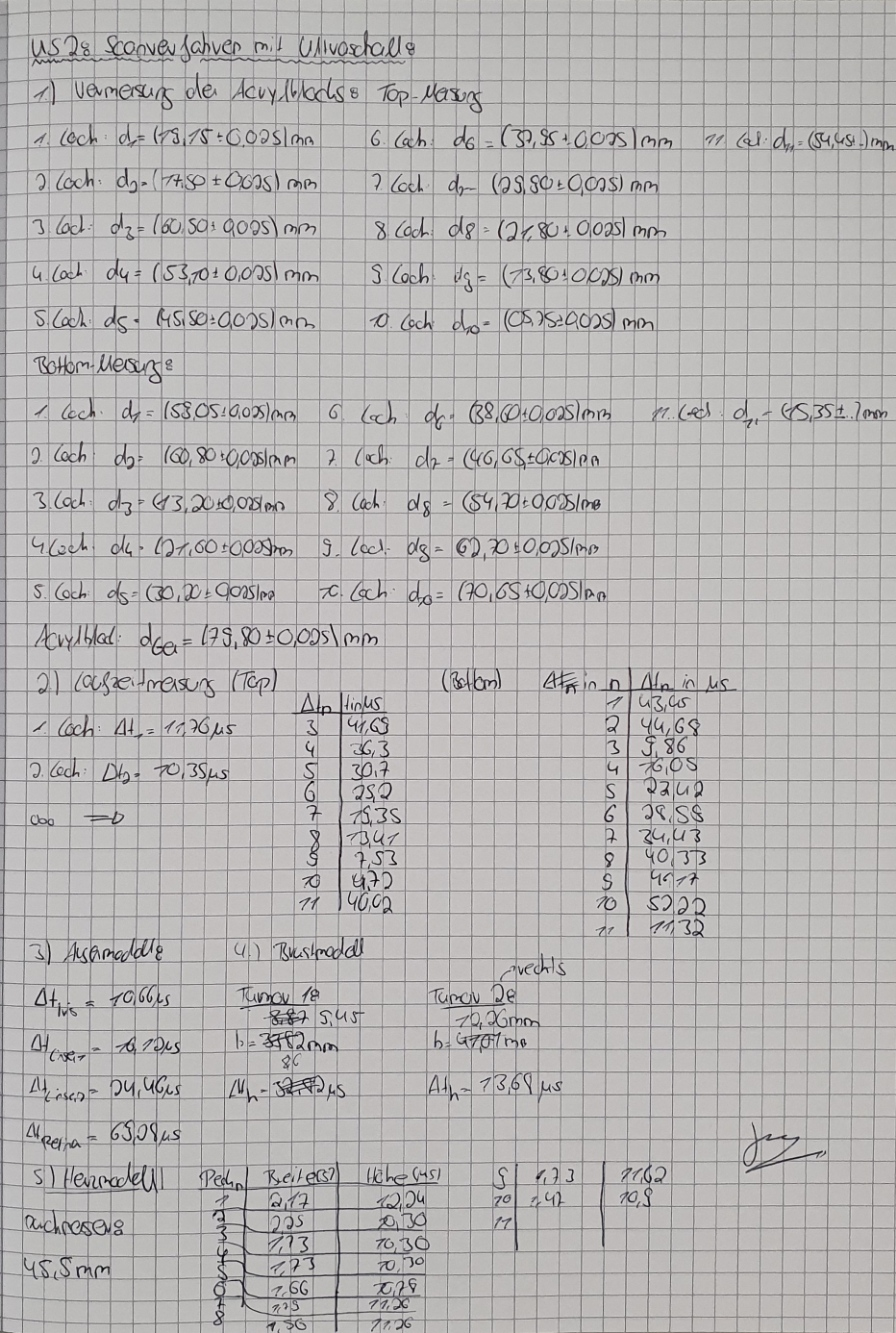
\includegraphics[width=0.9\textwidth]{content/20240521_115402.jpg}
    \caption{Laborbuch.}
\end{figure}


%Anpassungsschicht muss selbst bestimmt werden
%Geschwindigkeit über Tumore nocht konstant
%Schallgeschwindigkeit in wasser angenommen und nicht in silikon oder Tumor
%Reindrücken in Silikon verändert evtl auch Lage des Tumors
%Ultraschallsonde nicht immer orthogonal auf Brust
%Werte wie Größe des Tumors und Herzzeitvolumen von der Apparatur abhängig und daher keine Literaturwerte
%Messungen gut, da schallgeschwindigkeit 1% von Literaturwert abweicht


%\end{document}
